The hippocampus is a small organ with a seahorse-like shape that lies in the centre of the brain, right bellow the cortex (Figure~\ref{fig:brain:hippo}). It's part of the limbic system and it is thought to play a huge role in memory consolidation and spatial navigation.
The shape of the hippocampus is similar across mammals and its size increases with body size. There is also a relation between the size of the hippocampus and spatial memory. When compared in different species, the ones that present greater navigational abilities have larger hippocampi~\cite{jacobs2003evolution}. A similar phenomenon was found in humans, a study found that taxi drivers had an enlarged posterior section of the hippocampus when compared to the general public~\cite{taxi-maguire}.

\begin{figure}[h]
  \begin{center}
    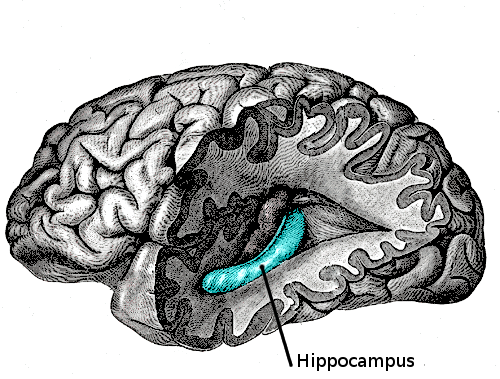
\includegraphics[width=0.5\textwidth]{Gray739-emphasizing-hippocampus}
    \caption{The cyan blob at the lower end of the diagram is the hippocampus~\cite{wikipedia-images}. }
    \label{fig:brain:hippo}
  \end{center}
\end{figure}

Studies of moving rodents have found that hippocampal neurons have preference for spatial and navigational features~\cite{okeefe1971hippocampus,milford2010robot}:
\begin{description}
  \item[Place cells.] They emit bursts of action potentials whenever the animal passes through a location in their environment. The environment that makes a place cell to fire is called a place field. Nonetheless, place cells' firing is also affected by other factors (e.g. visual cues, food location).
  \item[Head direction cells.] These cells react profusely to a preferred direction of the rodent's head. The firing rate seems to be independent of body direction, though some cells may be influenced by the animal's velocity.
  \item[Grid cells.] Neurons in this group increase their firing rate when the rodent is located in the intersection of a grid-like representation of the environment.
  \item[Border cells.] If a border that is large enough to modify the path of the rodent is present, this type of neurons will fire continuously.
\end{description}

\begin{figure}[h]
  \begin{center}
    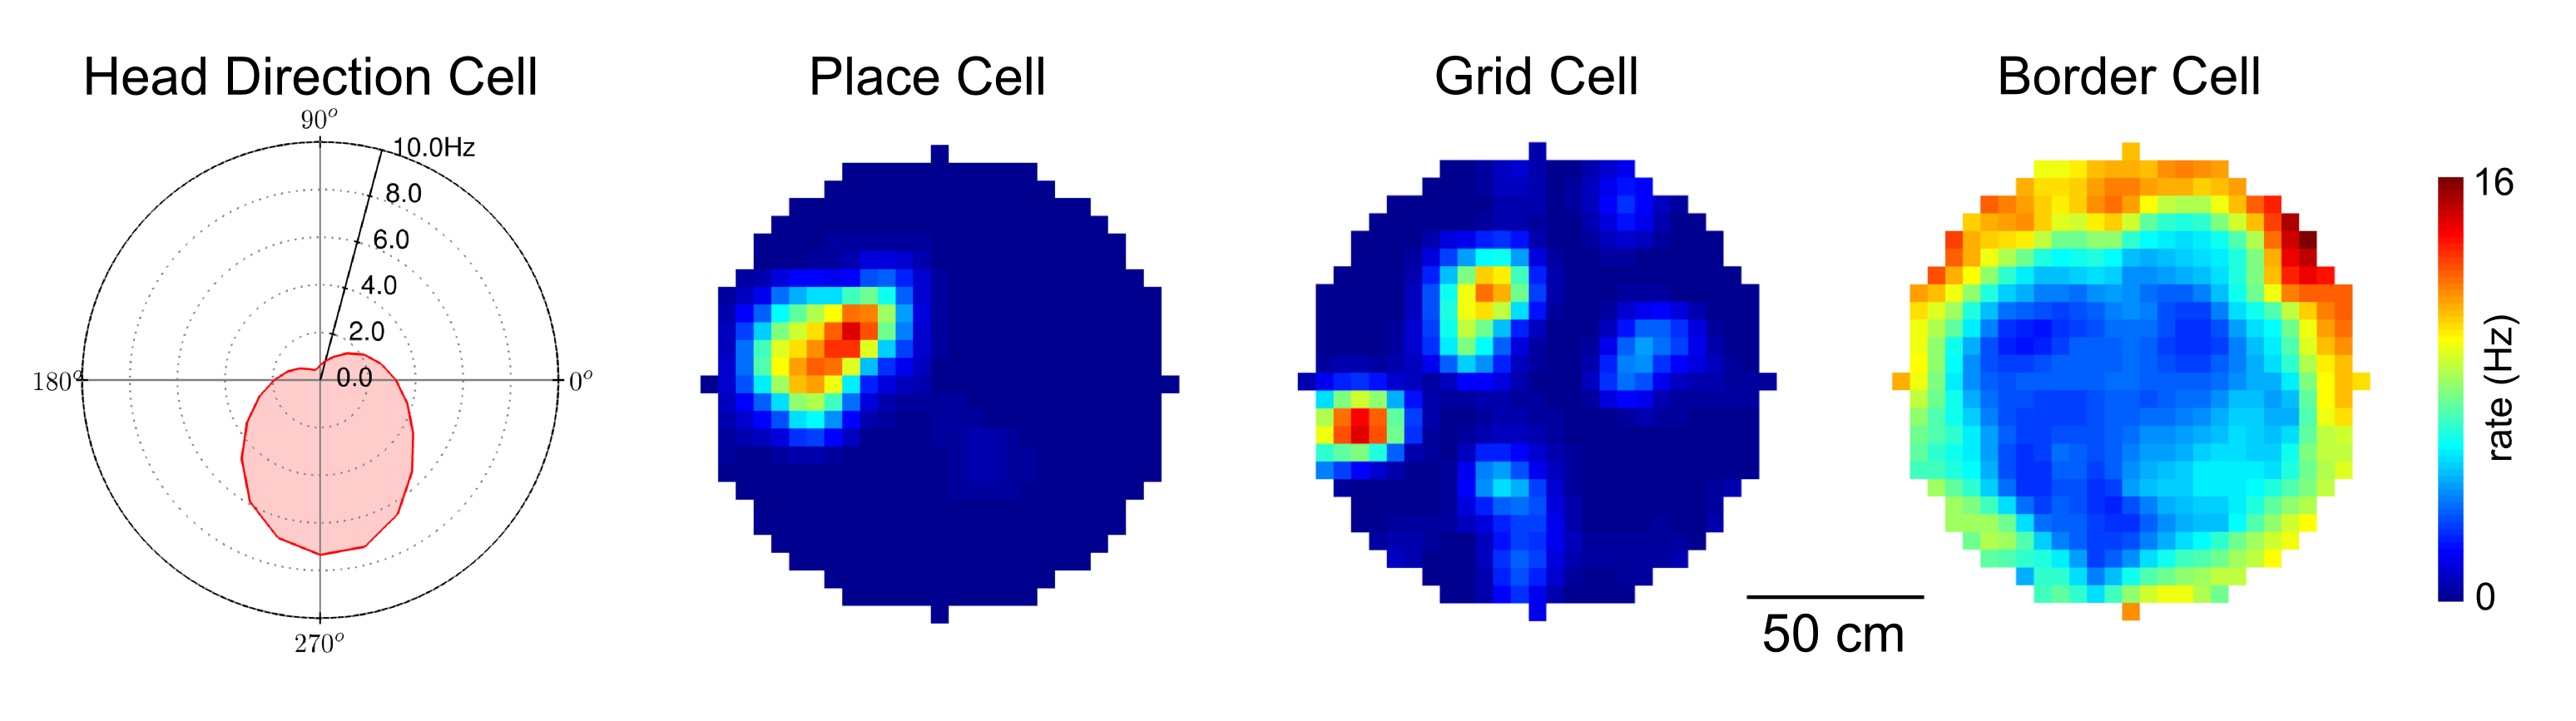
\includegraphics[width=0.7\textwidth]{cell_types_tuning1}
    \caption{Different hippocampal neuron's response to their preferred stimulus (adapted from~\cite{kloosterman-images}.)}
  \end{center}
\end{figure}

In primates, head direction cells' firing rate depends on direction of the head but not the direction of the eyes. Other work on primates, states that some hippocampal cells actually react to where the animal is looking, these are known as \emph{spatial view cells}~\cite{rolls2006spatial}. This evidence suggests that, one of the functions of the hippocampus might be to act as a cognitive map of the environment. 

%Episodic memories for nav